% !TeX root = Bachelorarbeit.tex
\chapter{Frontend}
\label{Frontend}

\section{Aufbau}

\begin{figure}[htbp] 
  \centering
     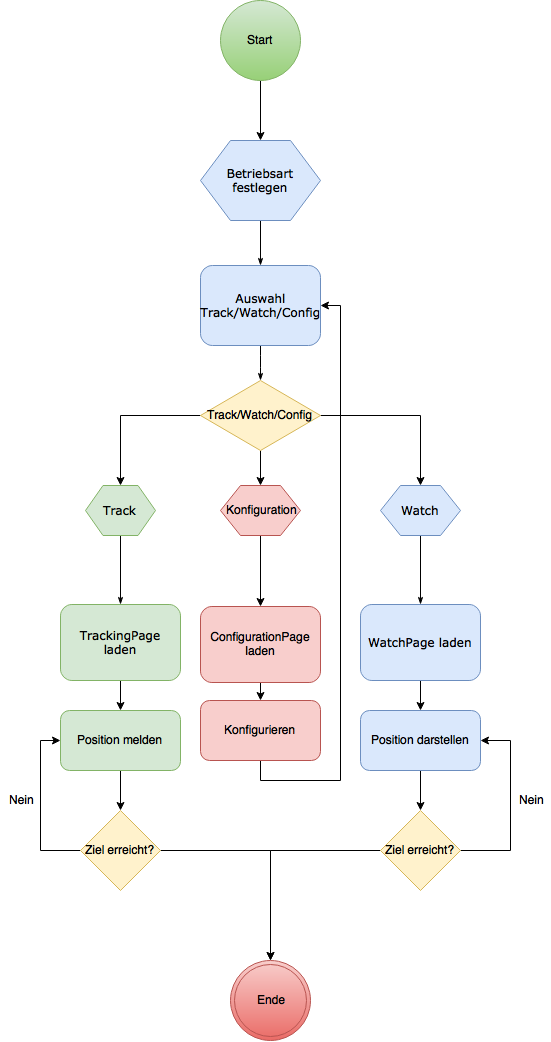
\includegraphics[width=0.7\textwidth]{images/FlowChart_Bustracker.png} 
  \caption{Ablaufdiagramm \emph{Bustracker}}
  \label{fig:Ablaufdiagramm}
\end{figure}


Die App gliedert sich in folgende Bereiche:
\begin{description}
\item[Watch Bereich] \hfill \\
Im Watch Bereich lädt die App regelmäßig Daten des zu beobachtenden Nutzers von einem Server. 
\item[Track Bereich] \hfill \\
Im Track Bereich führt die App regelmäßig Positionsbestimmungen durch und wartet auf das Entdecken bestimmter iBeacons durch das Gerät. So erkennt die App Checkpoints, in der Regel Haltestellen oder Ziele. 
\item[Konfiguration] \hfill \\
In der Konfiguration wird festgelegt, welcher Nutzer beobachtet wird. In Zukunft wird diese Konfiguration komplexer und umfangreicher werden.
\end{description}


\section{Funktionsweise}

Bei erstmaligem Start werden die sogenannten Permissions abgefragt. Der Nutzer muss der App den Zugriff auf Festspeicher, Bluetooth und \gls{gls:gps} gestatten. Dann gelangt der Nutzer auf die \nameref{HomePage}. Hier wählt der Nutzer aus, ob er seinen Standort mitteilen oder ein anderes Gerät verfolgen möchte. Nur von der Homepage kommt der Nutzer auf die \nameref{ConfigurationPage}. Dort stellt der Nutzer seine eigene ID (die UserID), sowie die ID des zu beobachtenden Geräts (trackingID) ein, anschließend kehrt er auf die \nameref{HomePage} zurück. Abbildung \ref{fig:Ablaufdiagramm} zeigt die App in Form eines Ablaufdiagramms. 



\subsection{API}
\label{API}
Das Akronym \gls{gls:API} steht für \emph{Application Programming Interface} und bedeutet Programmierschnittstelle. Sie definiert in welcher Form Daten, in diesem Fall serverseitig, angenommen und bereitgestellt werden. Sie stellt definierte Funktionen für den Datentransfer bereit. Ein großer Vorteil einer \gls{gls:API} besteht darin, dass sich die interne Datenverwaltung der \gls{gls:API} ändern kann, ohne die Schnittstelle zu beeinflussen.
Abbildung \ref{fig:API} zeigt den Kommunikationsablauf mit \emph{Bustracker}.
Die \gls{gls:API} ist nicht an die jeweilige Anwendung gebunden. Weitere Anwendungen könnten die \gls{gls:API} verwenden, um Daten bereitzustellen oder abzurufen. So wäre es denkbar, Skills für Sprachassistenten zu entwickeln, die auf die \gls{gls:API} Daten zurückgreifen. 

\begin{figure}[htbp] 
  \centering
     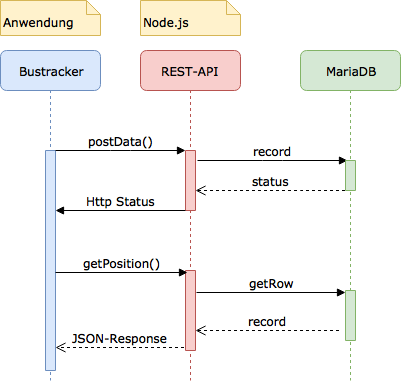
\includegraphics[width=0.7\textwidth]{images/APIsequence.png} 
  \caption{\emph{Bustracker} API Sequenzdiagramm}
  \label{fig:API}
\end{figure}

\emph{Bustracker} kommuniziert mit einer \gls{gls:rest} - \gls{gls:API} (siehe Kapitel \ref{REST}), dies ist eine gängige Form für \glspl{gls:API}. Zum Zeitpunkt der Entwicklung befand sich der Server innerhalb des hochschulinternen Netzwerks und war von außen nur per \gls{gls:VPN} zu erreichen. In einer Produktivumgebung wird der Server direkt erreichbar sein, dann mit einer Nutzerauthentifizierung.

\subsection{Speicherstruktur}
\begin{figure}[htbp] 
  \centering
     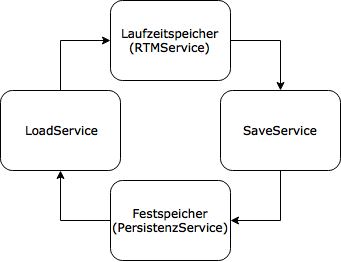
\includegraphics[width=0.7\textwidth]{images/Speicherstruktur.png} 
  \caption{\emph{Bustracker} Speicherstruktur mit Datenflussrichtung}
  \label{fig:Speicherstruktur}
\end{figure}

Die Struktur des Speichers (siehe Abb. \ref{fig:Speicherstruktur}) wurde so gewählt, dass der \nameref{srv:PersistenzService} keine anderen Injectables instantiiert. 
Der \nameref{srv:LoadService} und der \nameref{srv:SaveService} instantiieren den PersistenzService, der den Festspeicher des Geräts verwaltet. Load- und SaveService werden nur vom \nameref{srv:RTMService} instantiiert. Daraus ergibt sich eine Struktur, die unanfällig für Zirkelbezüge ist.   
Um einen Zirkelbezug, wie in Kapitel 6 aus dem Praxisbericht \cite{PraxBerJoSc} dargestellt zu vermeiden, wurde die Speicherstruktur direkt so ausgestaltet, dass sich keine Injectables gegenseitig instantiieren.
 

